\documentclass[conference]{IEEEtran}
\IEEEoverridecommandlockouts
% The preceding line is only needed to identify funding in the first footnote. If that is unneeded, please comment it out.
\usepackage{cite}
\usepackage{amsmath,amssymb,amsfonts}
\usepackage{algorithmic}
\usepackage{graphicx}
\usepackage{textcomp}
\usepackage{xcolor}
\def\BibTeX{{\rm B\kern-.05em{\sc i\kern-.025em b}\kern-.08em
    T\kern-.1667em\lower.7ex\hbox{E}\kern-.125emX}}
\begin{document}

\title{Implementation and Evaluation of Differential Evolution Algorithm on CPU and GPU by using CUDA\\
% {\footnotesize \textsuperscript{*}Note: Sub-titles are not captured in Xplore and should not be used}
}

\author{\IEEEauthorblockN{Ali Khudiyev}
\IEEEauthorblockA{\textit{Data Science and Artificial Intelligence} \\
\textit{French-Azerbaijani University}\\
Baku, Azerbaijan \\
ali.khudiyev@ufaz.az}
}

\maketitle

\begin{abstract}
	Differential Evolution is one of the promising algorithms that is used for the various optimization problems. It has a huge potential to be run on Graphics Processing Units (GPUs)
	since the algorithm uses single instruction(i.e., mutation, crossover) on multiple data(i.e., vectors). In this paper, sequential and concurrent versions of DEA are developed and evaluated
	to compare and understand the trade-offs. Specific implmentation details such as algorithm architecture and optimization for CPU and GPU are discussed after introducing general theory of DEA.
	Experiments are carried on several times with the algorithm termination criteria of maximum number of objective function evaluations and statistical data are presented for both versions of the algorithm.
	Results are discussed in terms of the presented statistical data and finally, I come to the conclusion that which version of the DEA is to be used under certain conditions.
\end{abstract}

\begin{IEEEkeywords}
	Optimization, Differential Evolution, CPU, GPU, CUDA
\end{IEEEkeywords}

\section{Introduction}
Differential Evolution is one of the many metaheuristics used for various optimization problems. Main goal of the algorithm is to find global minimum of a given $n$-dimensional function by performing 
3 operations on the randomly initialized list of points or population. The main problem that we may encounter while using such type of algorithms, is that the algorithm may get stuck in a local minimum,
in other words, we have to avoid premature convergence in order to get the global minimum. However, DEA is very handy and flexible for various number of optimization problems since it has no assumptions 
or restrict constraints for the problem it is applied to. Another benefit of using differential evolution comes from its nature; the algorithm is highly parallelizable as the performed operations are 
independent.

Implemention of sequential DEA on a CPU benefits the high speed of single core floating point calculations, however, true nature of the algorithm is not exploited due to sequentiality. For the latter 
purpose, one could utilize GPGPUs that have many cores compared to CPUs. Using GPUs efficiently is also tricky due to several concepts:

\begin{enumerate}
	\item Limited memory capcity and memory bandwidth
	\item Optimal utilization of shared and global memory
	\item Optimal schedule for limited number of SPs\footnote{Streaming Processor}
\end{enumerate}

GPUs have memory components with many streaming processors that enable hardware/software parallelism. The common parallelism exploited by such GPUs are by performing Single Instruction Multiple Data (SIMD) 
operations. Such instructions are needed when there are potentially vast amount of data elements that need go through same instruction execution pipeline. Obvious example of such computation paradigm is 
video games and graphics rendering. Two types of memory are common on GPUs: \textit{global} and \textit{shared}. Global memory is accessible for all processing units with low bandwidth and high capacity 
whereas shared memory is only accessible to a subset of them with high bandwidth and low capacity.

Graphics rendering or video games are not the only type of applications that may benefit from parallelism, in fact, all GPUs do, is vast amount of number crunching which can be handy for some scientific 
computations. However, we cannot just tell GPUs what to do without any specification or application programming interface (API). In previous years, OpenGL was the only option to write and execute 
programs on GPUs, but it was hard to use for scientific work since all the specification was built on pixel rendering paradigm. So, to do a scientific work on GPUs, one would need to transform the 
scientific calculations to some pixel-level calculations. Later on, NVIDIA developed Compute Unified D A (CUDA) which enabled programmers to execute instructions on GPUs more easily in a programmer-friendly 
way. To execute a program on a GPU by using CUDA, we need to use C-like language called CUDA-C.

\subsection{CUDA}

\begin{figure}[h]
	\centering
	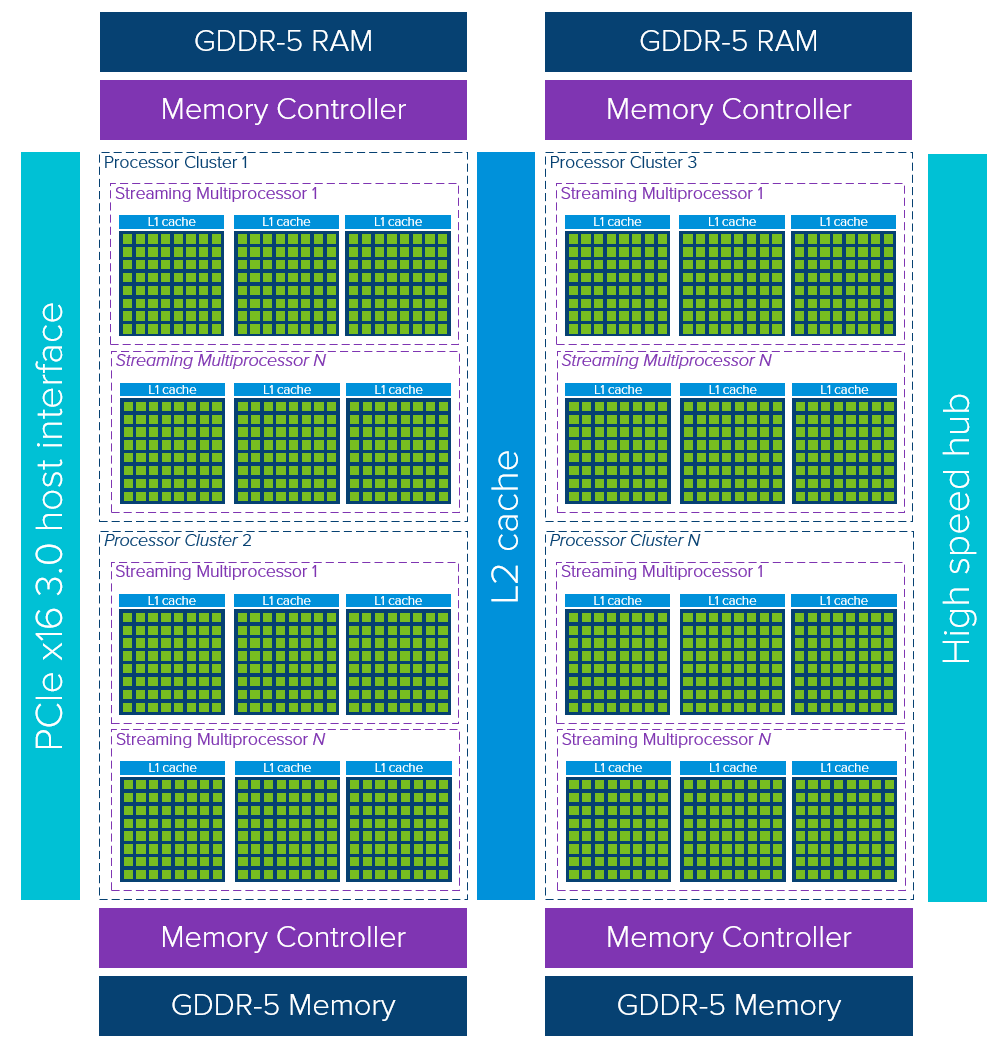
\includegraphics[width=0.75\linewidth]{img/gpu-architecture.png}
	\caption{GPU architecture}
	\label{fig:gpu_arch}
\end{figure}

Figure \ref{fig:gpu_arch}\footnote{https://core.vmware.com/resource/exploring-gpu-architecture} illustrates comman GPU architecture that has several processor clusters each of which containing several 
streaming multiprocessors that have shared L2 cache. Each streaming multiprocessor also contains several streaming processors with L1 caches.

\section{Sequential DEA Optimization}
Implementation of Differential Evolution algorithm on CPUs is straight forward for many educational cases. However, it requires relatively more knowledge of underlying working principles of CPU/GPUs and 
their architectures to be able to use all of what the modern technology offers in terms of power and efficiency. There are many implementation principles such as pass-by-reference 
(to reduce memory operations, instead of pass-by-value), dynamic programming (DP) (to reduce memory operations), single instruction multiple data (SIMD) operations 
(to reduce computation time, instead of SISD) and so on.

\subsection{Overview of DEA}

\subsubsection{Mutation}

\begin{equation}
	v_i = 
	\begin{cases}
		0, &h \\
		1, &v
	\end{cases}
	\label{Mutation operation}
\end{equation}

\subsubsection{Crossover}

\begin{equation}
	v_i = 
	\begin{cases}
		0, &h \\
		1, &v
	\end{cases}
	\label{Crossover operation}
\end{equation}

\subsubsection{Selection}

\begin{equation}
	v_i = 
	\begin{cases}
		0, &h \\
		1, &v
	\end{cases}
	\label{Selection operation}
\end{equation}

\section{Parallel DEA with CUDA}
\dots

\subsection{Proposed architecture for GPU version of DEA}
\dots

\section{Experiments}
\dots

\section{Results and Discussions}
\dots

\section{Conclusion}
\dots

% \section*{Acknowledgment}
% 
% The preferred spelling of the word ``acknowledgment'' in America is without 
% an ``e'' after the ``g''. Avoid the stilted expression ``one of us (R. B. 
% G.) thanks $\ldots$''. Instead, try ``R. B. G. thanks$\ldots$''. Put sponsor 
% acknowledgments in the unnumbered footnote on the first page.

\section*{References}

Please number citations consecutively within brackets \cite{b1}. The 
sentence punctuation follows the bracket \cite{b2}. Refer simply to the reference 
number, as in \cite{b3}---do not use ``Ref. \cite{b3}'' or ``reference \cite{b3}'' except at 
the beginning of a sentence: ``Reference \cite{b3} was the first $\ldots$''

Number footnotes separately in superscripts. Place the actual footnote at 
the bottom of the column in which it was cited. Do not put footnotes in the 
abstract or reference list. Use letters for table footnotes.

Unless there are six authors or more give all authors' names; do not use 
``et al.''. Papers that have not been published, even if they have been 
submitted for publication, should be cited as ``unpublished'' \cite{b4}. Papers 
that have been accepted for publication should be cited as ``in press'' \cite{b5}. 
Capitalize only the first word in a paper title, except for proper nouns and 
element symbols.

For papers published in translation journals, please give the English 
citation first, followed by the original foreign-language citation \cite{b6}.

\begin{thebibliography}{00}
\bibitem{b1} G. Eason, B. Noble, and I. N. Sneddon, ``On certain integrals of Lipschitz-Hankel type involving products of Bessel functions,'' Phil. Trans. Roy. Soc. London, vol. A247, pp. 529--551, April 1955.
\bibitem{b2} J. Clerk Maxwell, A Treatise on Electricity and Magnetism, 3rd ed., vol. 2. Oxford: Clarendon, 1892, pp.68--73.
\bibitem{b3} I. S. Jacobs and C. P. Bean, ``Fine particles, thin films and exchange anisotropy,'' in Magnetism, vol. III, G. T. Rado and H. Suhl, Eds. New York: Academic, 1963, pp. 271--350.
\bibitem{b4} K. Elissa, ``Title of paper if known,'' unpublished.
\bibitem{b5} R. Nicole, ``Title of paper with only first word capitalized,'' J. Name Stand. Abbrev., in press.
\bibitem{b6} Y. Yorozu, M. Hirano, K. Oka, and Y. Tagawa, ``Electron spectroscopy studies on magneto-optical media and plastic substrate interface,'' IEEE Transl. J. Magn. Japan, vol. 2, pp. 740--741, August 1987 [Digests 9th Annual Conf. Magnetics Japan, p. 301, 1982].
\bibitem{b7} M. Young, The Technical Writer's Handbook. Mill Valley, CA: University Science, 1989.
\end{thebibliography}

\end{document}
